\subsection{Product Perspective}
% Introductory text describing system's integration with other products, considering shared phenomena.

% Text for Class Diagram
% Class diagram

% TODO: @Ozan If have time start this.

% For each core feature (which are they? all?):
%   - Scenario
%   - State Chart
%   - Explanation

% TODO: @Ozan go with these.
% Core features: Future book line number, now retrieve line number, Guest arrives to store, System stop (Shop's on fire), schedule system stop (don't forget to notify customer),
\subsubsection{Book Line Number}
\textbf{Scenario}

\textbf{State Chart}

\begin{figure}[H]
    \centering
    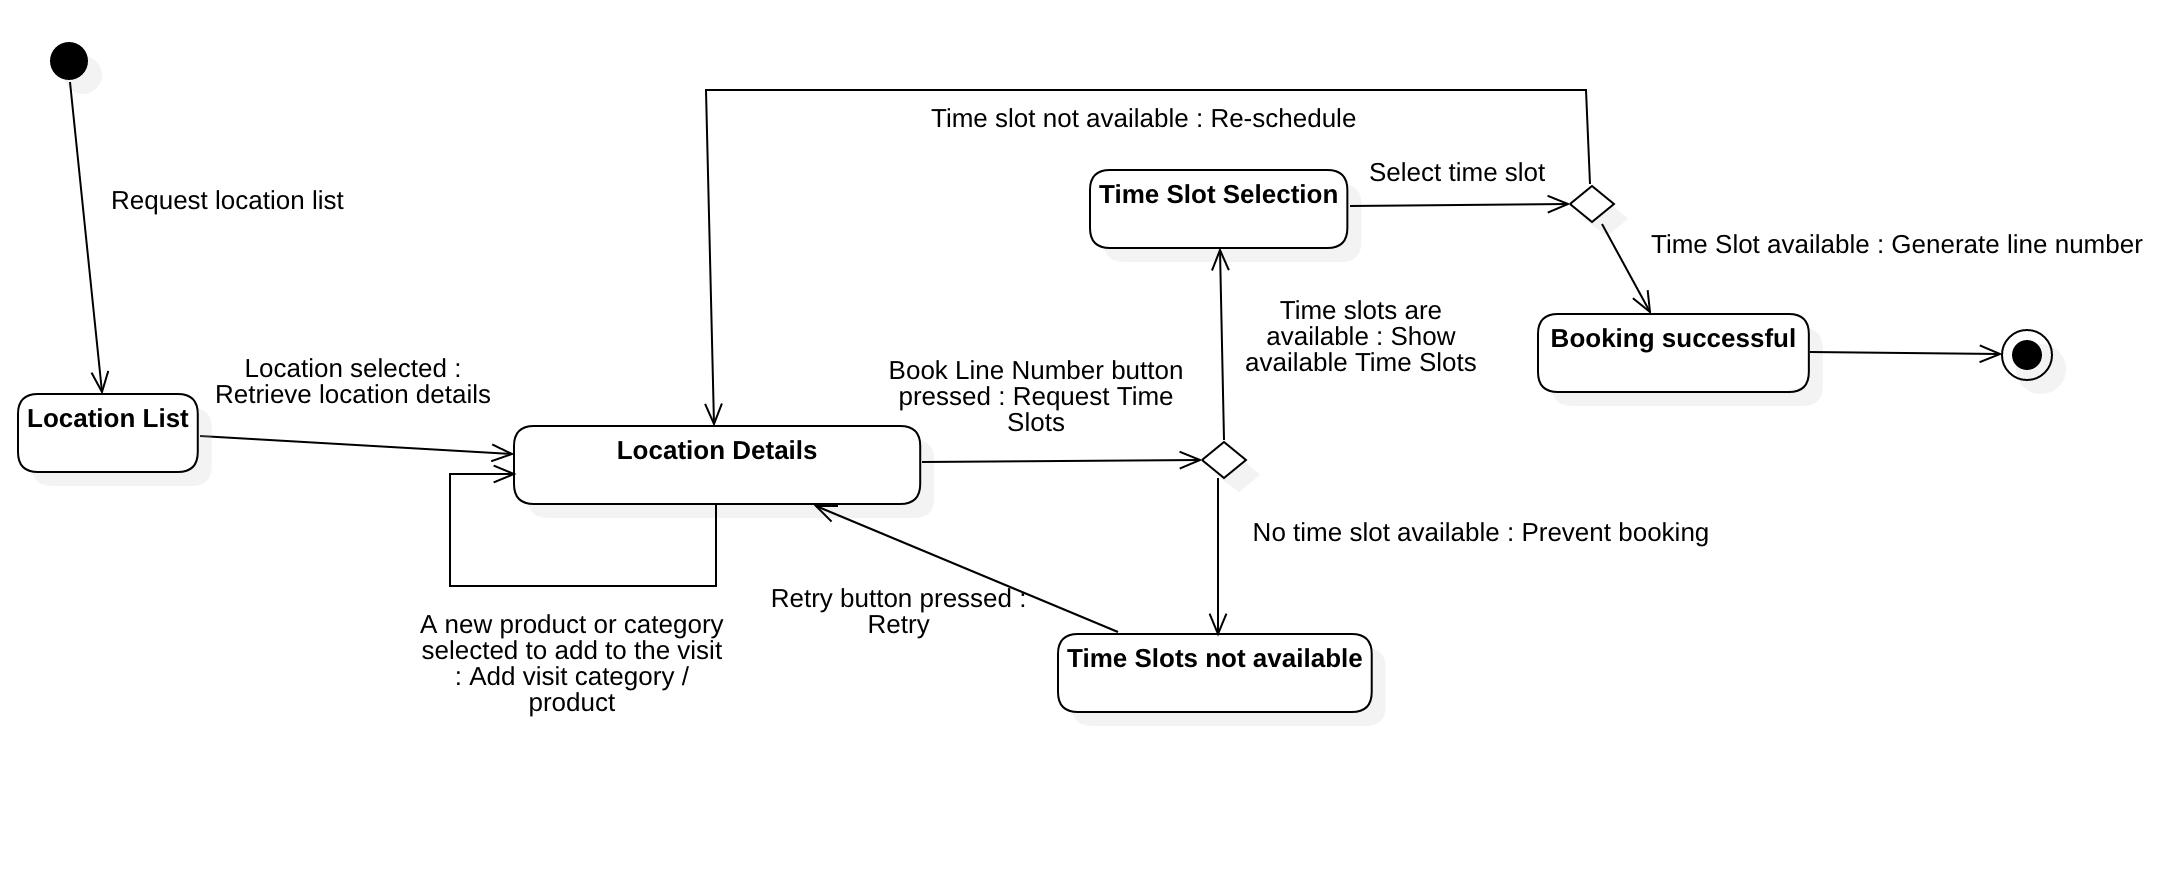
\includegraphics[height=0.4\textwidth]{Images/StateCharts/BookLineNumber.png}
    \caption{State Diagram for feature Book Line Number}
\end{figure}
\subsubsection{Get Line Number}

\textbf{Scenario}

\textbf{State Chart}
\begin{figure}[H]
    \centering
    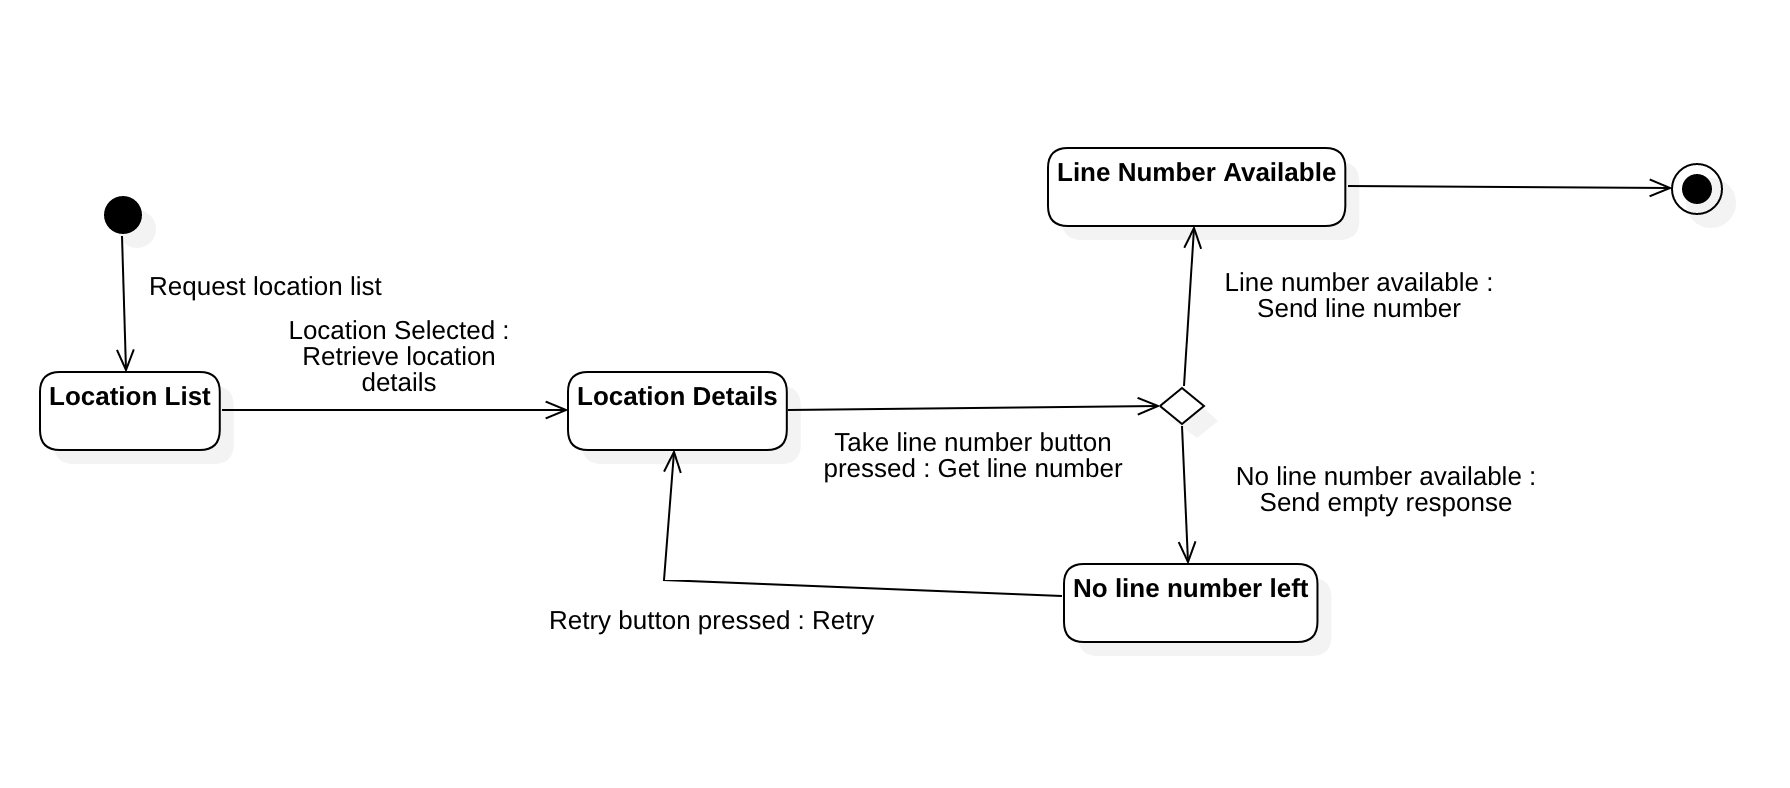
\includegraphics[height=0.4\textwidth]{Images/StateCharts/GenerateLineNumber.png}
    \caption{State Diagram for feature Get Line Number}
\end{figure}
\subsubsection{Print Line Number}

\textbf{Scenario}

\textbf{State Chart}
\begin{figure}[H]
    \centering
    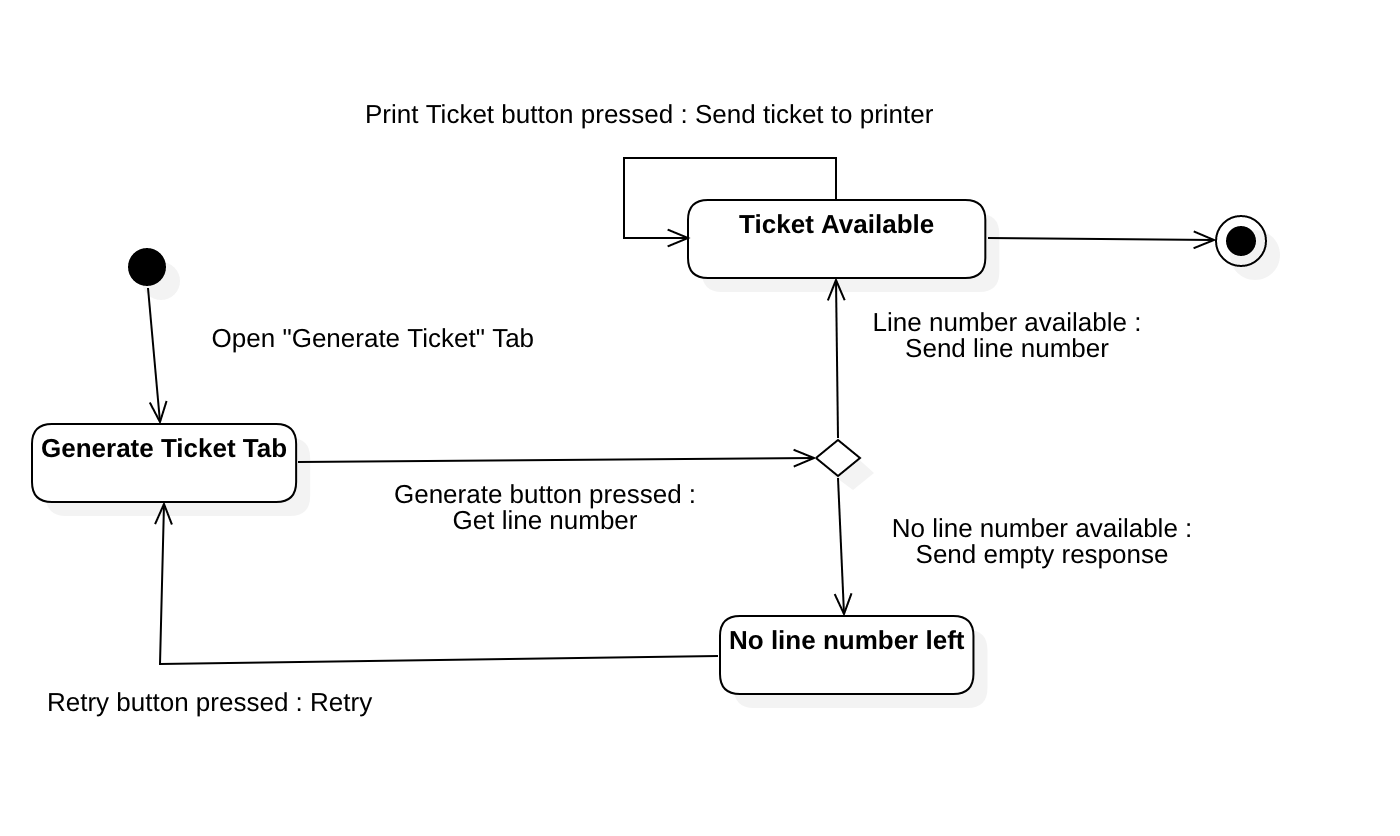
\includegraphics[height=0.4\textwidth]{Images/StateCharts/PrintTicket.png}
    \caption{State Diagram for feature Print Line Number}
\end{figure}
\subsubsection{System Stop}

\textbf{Scenario}

\textbf{State Chart}
\begin{figure}[H]
    \centering
    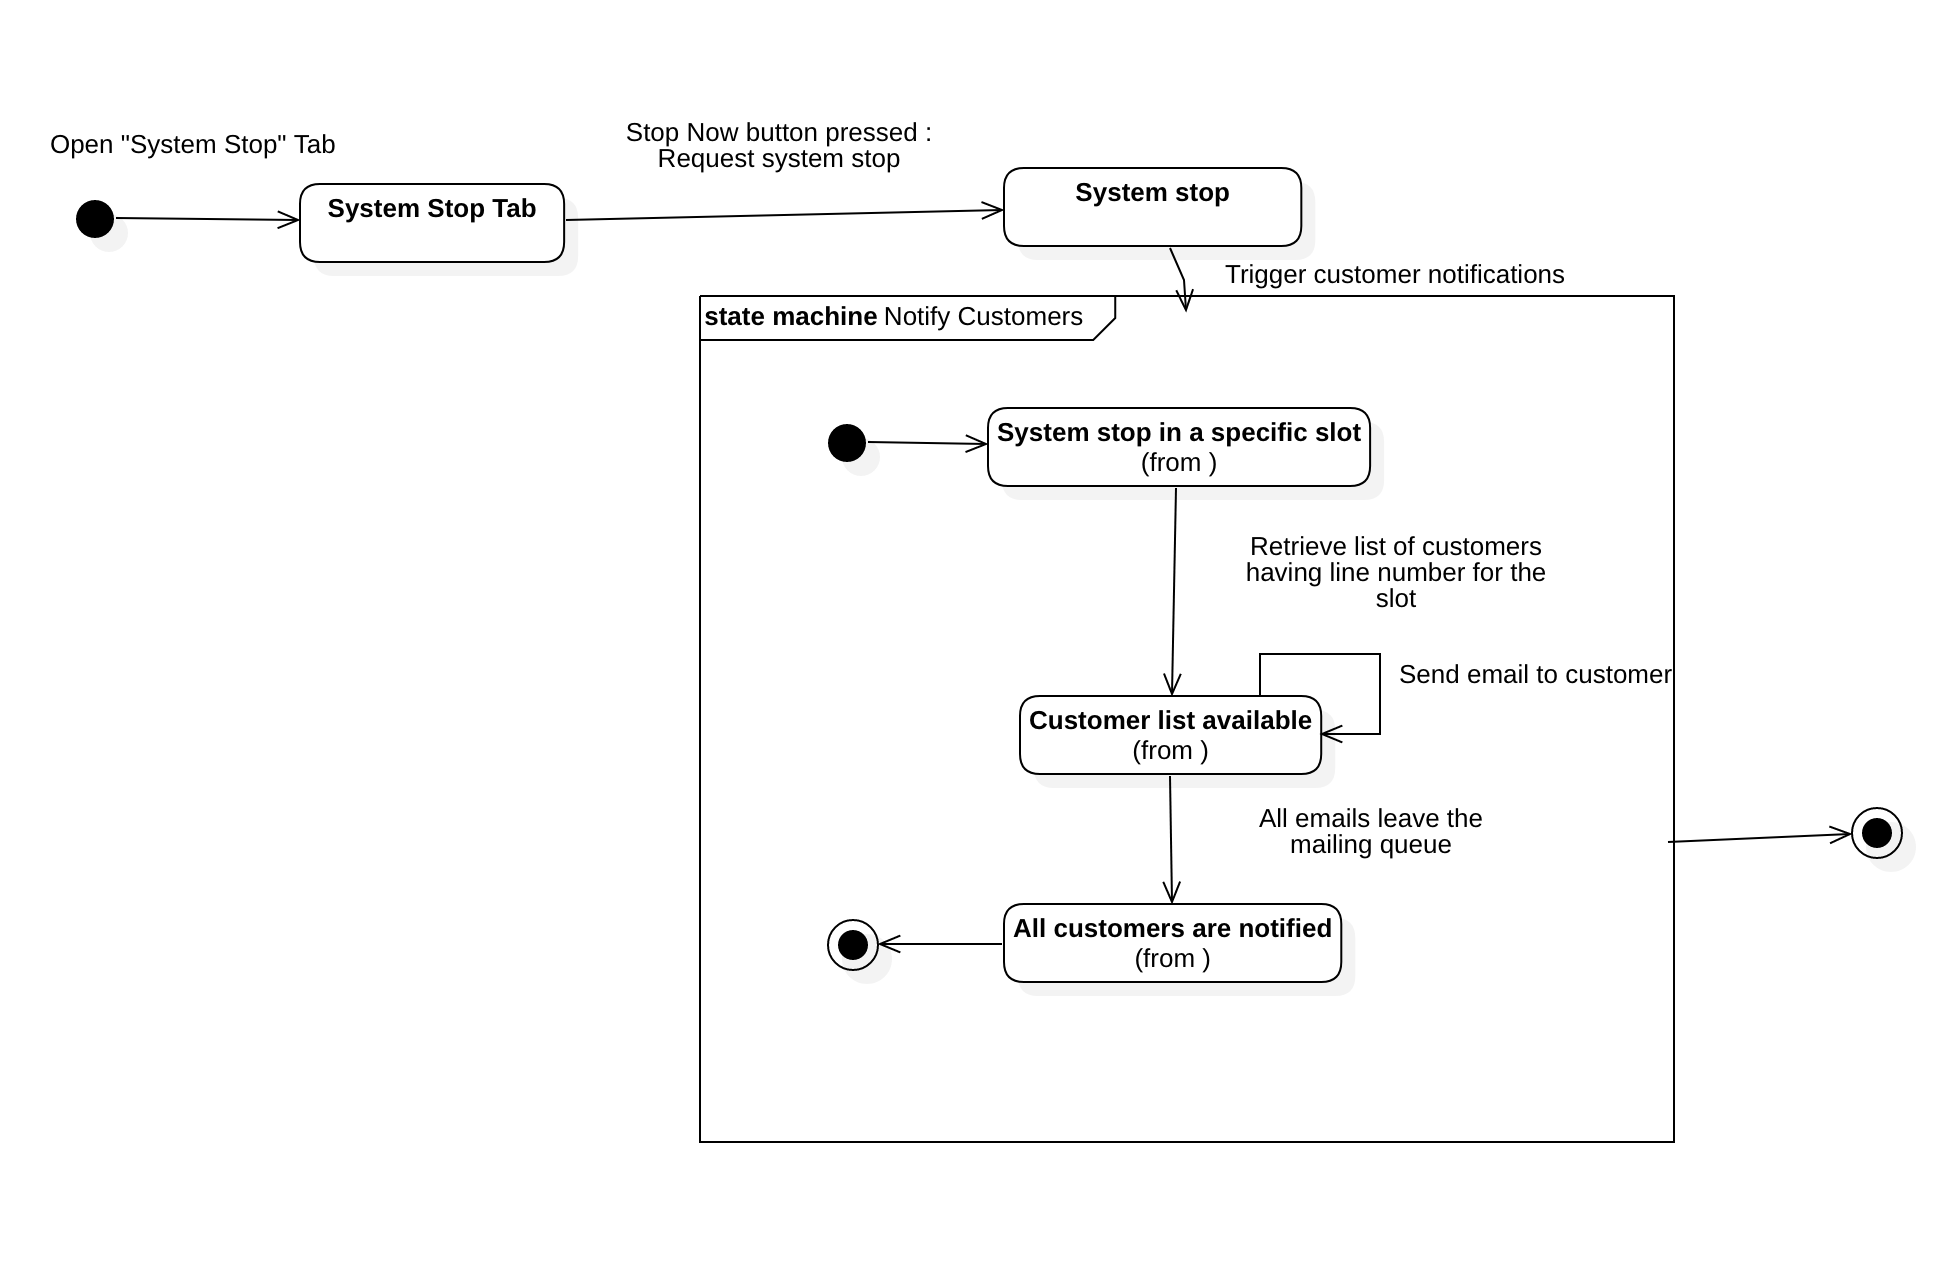
\includegraphics[height=0.4\textwidth]{Images/StateCharts/SystemStop.png}
    \caption{State Diagram for feature System Stop}
\end{figure}

\subsubsection{Schedule System Stop}

\textbf{Scenario}

\textbf{State Chart}
\begin{figure}[H]
    \centering
    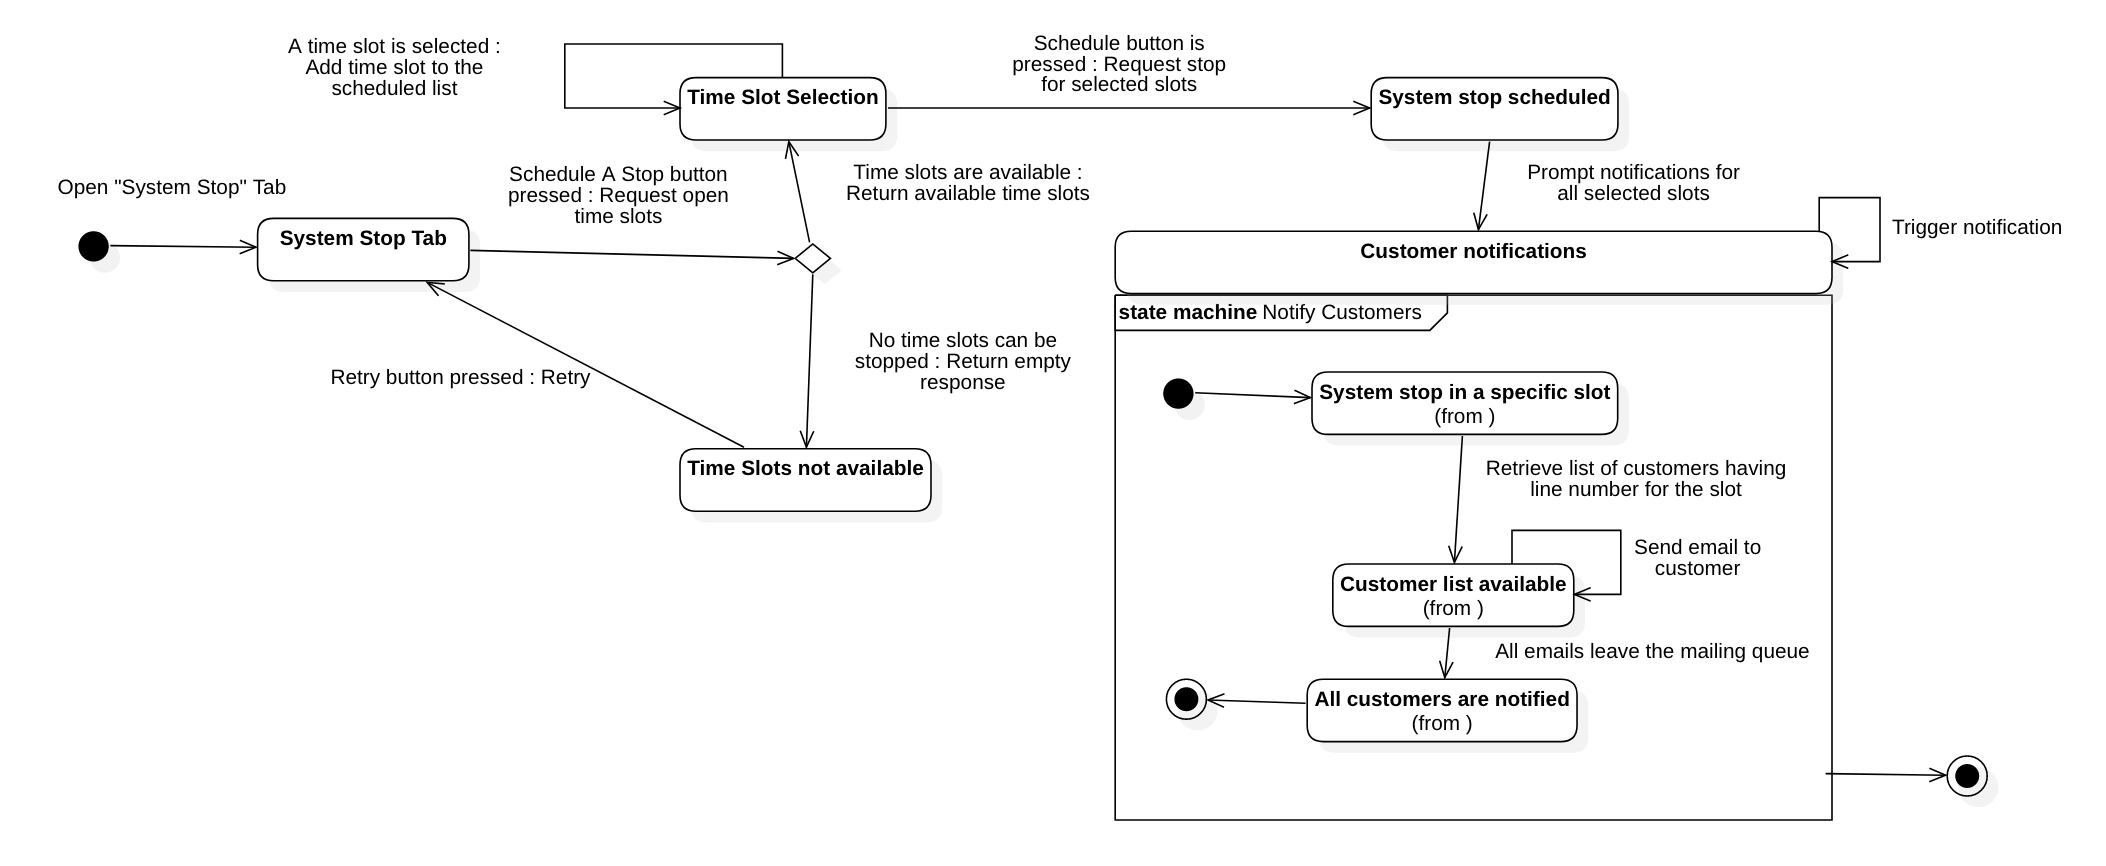
\includegraphics[height=0.4\textwidth]{Images/StateCharts/ScheduleSystemStop.png}
    \caption{State Diagram for feature Schedule System Stop}
\end{figure}
% here  we  include scenarios  and further details on the shared phenomena and a domain model (class diagrams and state charts)


\subsection{Product functions}
% TODO: @Hrvoje do these 3

% subsubsections with functions of (some?) requirements
% here we include the most important requirements
% for requirements use the R_1, R_2, R_3 syntax


\subsection{User characteristics}
% User roles: Manager & User & Clerk (& maybe unregistered user?)

% People need to be able to use Tickets, maybe: %90 / %10
% here we include anything that is relevant to clarify their needs


\subsection{Assumptions,dependencies and constraints}
\subsubsection{Domain Assumptions}

\begin{itemize}
    \item \textbf{$D_1$} \%80 of the customers and all clerks and managers have basic ICT skills, has an email address that they are willing to use to authenticate to the system and has a smart phone or equivalent device that can connect to the Internet, have a browser that supports UTF-8, display QR codes and has a mapping application. % All cases
    \item \textbf{$D_2$} Locations will not be visited by no more than 1000 people in any time slot. % Line number limit, we can provide 000-999 as numbers
    \item \textbf{$D_3$} \%98 of the customers will arrive at the given location either without a ticket or with a ticket that has not timed out. % Timeout policy
    \item \textbf{$D_4$} E-mail addresses are not shared by multiple users of the system. % Registeration, user info
    \item \textbf{$D_5$} Clerks' mobile devices are equipped with at least one camera that the system can use. % For QR code detection
    \item \textbf{$D_6$} All users have a basic understanding of how the line numbering system works and respects the ordering provided by the system. % The core use case
    \item \textbf{$D_7$} Managers have an estimate for the amount of reservations that their location can at most have. % To set a maximum amount of clients
    \item \textbf{$D_8$} Managers' device has location services that has a location acquisition error for no more than 20 meters. % To set the location accurately
    \item \textbf{$D_9$} Clerks are constantly monitoring the locations entrances and exits. % For QR code reading to take customers in and out
    \item \textbf{$D_{10}$} Locations have printing equipments that are in 5 meters range of all the entrances that can print QR codes and line numbers. % To print tickets
    \item \textbf{$D_{12}$} At least one manager is available in the location during the working hours. % To monitor and shutdown during emergencies
    \item \textbf{$D_{13}$} The customer's entry and exit to the store is determined by whether the clerks have checked them in and out.
    \item \textbf{$D_{14}$} The customer has their line number or line number ticket available with them through their visit, including their exit from the store % (no dead battery, printed ticket loss, etc)
\end{itemize}
% here we include domain assumptions
% use the D_1, D_2,... syntax
\subsubsection{Dependencies}
% TODO: @Hrvoje these 2 too.
% Maps API
% What external libraries, tools, integrations does the system rely on
\subsubsection{Constraints}
% Maps API failure
% All user and location info can be represented with UTF-8 character encoding.
% What are the limits imposed by the environment, regulatory policies, hardware & software limitations, etc...
